
\documentclass[12pt]{article}
%\topmargin=-0.5in
%\textheight=9in
%\evensidemargin=0in
%\oddsidemargin=0in
%\setlength{\textwidth}{6.5in}

\usepackage{amsmath,latexsym}
\usepackage{amsfonts}
\usepackage{amssymb}
\usepackage{amssymb}
\usepackage{caption}
\usepackage{graphicx}
%\usepackage{appendix}
%\usepackage{clrscode3e}
\usepackage{epstopdf}
\usepackage{subfigure}
%\usepackage{algorithm}
%\usepackage{algorithmic}
\usepackage{setspace}
\usepackage{color}
\usepackage{listings}
\usepackage{setspace}
\usepackage{algpseudocode}
\usepackage{algorithm}
\usepackage[all]{xy}
\usepackage{pdfpages}
% \doublespacing
\renewcommand{\topfraction}{0.9}	% max fraction of floats at top
\renewcommand{\bottomfraction}{0.8}	% max fraction of floats at bottom
%   Parameters for TEXT pages (not float pages):
\setcounter{topnumber}{2}
\setcounter{bottomnumber}{2}
\setcounter{totalnumber}{4}      % 2 may work better
\setcounter{dbltopnumber}{2}    % for 2-column pages
\renewcommand{\dbltopfraction}{0.9}	% fit big float above 2-col. text
\renewcommand{\textfraction}{0.07}	% allow minimal text w. figs
%   Parameters for FLOAT pages (not text pages):
    \renewcommand{\floatpagefraction}{0.7}	% require fuller float pages
% N.B.: floatpagefraction MUST be less than topfraction !!
\renewcommand{\dblfloatpagefraction}{0.7}	% require fuller float pages

\newenvironment{dig}{\\ [6pt]\noindent {\bf Digression}}{~$\Box$\\ [6pt]\indent}
\newenvironment{dig1}{\noindent {\bf Digression}}{~$\Box$\\ [6pt]\indent}
\newtheorem{alg}{\hspace{1.3in} Algorithm}
\newtheorem{thrm}{Theorem}
\newtheorem{lemm}[thrm]{Lemma}
\newtheorem{conj}[thrm]{Conjecture}
%\newtheorem{claim}[thrm]{Claim}
\newtheorem{prop}[thrm]{Proposition}
\newtheorem{defn}[thrm]{Definition}
\newtheorem{obs}[thrm]{Observation}

\hyphenation{Chris-to-dou-lak-is}
\def\proof{\bigbreak\noindent {\sl Proof.\/}\enspace}
\def\qedbox#1#2{\vbox{\hrule height.2pt
  \hbox{\vrule width.2pt height#2pt \kern#1pt \vrule width.2pt}
  \hrule height.2pt}}
\def\qed{\hfill \quad\qedbox46\newline\smallbreak}

\def\s#1{\mbox{\boldmath $#1$}}
\def\floor#1{\lfloor #1 \rfloor}
\def\bfloor#1{\big\lfloor #1 \big\rfloor}
\def\Bfloor#1{\Big\lfloor #1 \Big\rfloor}
\def\ceil#1{\lceil #1 \rceil}
\def\bceil#1{\big\lceil #1 \big\rceil}
\def\+{\!+\!}
\def\-{\!-\!}
\def\plmi{\!\pm\!}
\def\m{\!-\!}
\def\uu#1{\underline{#1}}
\def\o#1{\overline{#1}}
\def\itbf#1{\textit{\textbf{#1}}}
\def\match{\approx}
\def\cP{\mathcal{P}}
\def\G{\mathcal{G}}
\def\B{\mathcal{B}}
\def\O{\mathcal{O}}

\def\bproc{{\bf procedure\ }}
\def\bfunc{{\bf function\ }}
\def\bvar{{\bf var\ }}
\def\barray{{\bf array\ }}
\def\bof{{\bf of\ }}
\def\bfor{{\bf for\ }}
\def\bnull{{\bf null\ }}
\def\bto{{\bf to\ }}
\def\bdownto{{\bf downto\ }}
\def\bwhile{{\bf while\ }}
\def\brep{{\bf repeat\ }}
\def\buntil{{\bf until\ }}
\def\band{{\bf and\ }}
\def\bor{{\bf or\ }}
\def\bdo{{\bf do\ }}
\def\bif{{\bf if\ }}
\def\bthen{{\bf then\ }}
\def\belse{{\bf else\ }}
\def\belsif{{\bf elsif\ }}
\def\bnot{{\bf not\ }}
\def\bgoto{{\bf goto\ }}
\def\bcontinue{{\bf continue\ }}
\def\breturn{{\bf return\ }}
\def\bbreak{{\bf break\ }}
\def\boutput{{\bf output}}
\def\la{\leftarrow}
\def\ra{\rightarrow}
\def\llra{\Leftrightarrow}
\def\q{\quad}
\def\qq{\qquad}
\def\com#1{{\bf $\triangleright$}\hspace{6pt}{\sl #1}}
\def\rem#1{\hspace{24pt}{\sl #1}}
\def\pref(#1,#2){$#1$ is a prefix of $#2$}
\def\suff(#1,#2){$#1$ is a suffix of $#2$}
\def\FIND{\mbox{FIND}}
\def\reg(#1,#2){$#2$ is $#1$-regular}
\def\notreg(#1,#2){$#2$ is not $#1$-regular}
\def\top{\tt{top}}
\def\pop{\tt{pop}}
\def\push{\tt{push}}
\def\true{\tt{true}}
\def\false{\tt{false}}
\def\UPDATE\_F{\tt{UPDATE\_F}}
\def\LEAST{\tt{LEAST}}
\def\MERGE{\tt{MERGE}}
\def\mec{\tt{mec}}
\def\MEC{\tt{MEC}}
\def\CMEC{\tt{CMEC}}
\def\MELC{\tt{MELC}}
\def\CMELC{\tt{CMELC}}
\def\MELS{\tt{MELS}}
\def\CMELS{\tt{CMELS}}
\def\MCNT{\tt{MaxCount}}
\def\CLEN{\tt{CorLen}}

% \def\B{\tt{B}}
\def\Q'{\tt{Q'}}
\def\CP{\tt{CP}}
\def\MNC{\tt{MNC}}
\def\PR{\tt{PR}}
\def\PRS{\tt{PRS}}
\def\CPR{\tt{CPR}}
% \def\POS{\tt{POS}}
\def\LEN{\tt{LEN}}
\newcommand{\dd}{\mathinner{\ldotp\ldotp}}

\newif\ifShow
\Showfalse
% MATH -----------------------------------------------------------
\newcommand{\norm}[1]{\left\Vert#1\right\Vert}
\newcommand{\abs}[1]{\left\vert#1\right\vert}
\newcommand{\set}[1]{\left\{#1\right\}}
\newcommand{\Real}{\mathbb R}
\newcommand{\eps}{\varepsilon}
\newcommand{\To}{\longrightarrow}
\newcommand{\BX}{\mathbf{B}(X)}
\newcommand{\A}{\mathcal{A}}
% Algorithm ------------------------------------------------------

\algnewcommand{\LineComment}[1]{\State \(\triangleright\) \normalfont{\sl #1}}
\algtext*{EndWhile}% l
\algtext*{EndIf}% Remove "end if" text
\algtext*{EndFor}% Remove "end for" text
\algtext*{EndFor}% Remove "end for" text
\algtext*{EndProcedure}% Remove "end procedure" text

% manifold
\newcommand{\F}{{F}}
\newcommand{\scF}{\F}
\newcommand{\X}{{X}}
\newcommand{\Fhat}{\widehat\F}
\newcommand{\scN}{{\EuScript N}}
\newcommand{\scL}{{\EuScript L}}
\newcommand{\PP}{\mathbb P}
\newcommand{\R}{\mathbb R}
\newcommand{\C}{\mathbb C}
% \newcommand{\CP}{\C\PP}
\newcommand{\CH}{\C{\mathrm H}}
\newcommand{\Lie}{{\mathcal L}}
\newcommand{\cpn} {\CP^n}
\newcommand{\chn} {\CH^n}
\newcommand{\cptwo} {\CP^2}
\newcommand{\chtwo} {\CH^2}
\newcommand{\chone} {\CH^1}
%\newcommand{\mean}{{\mathcal m}}
\newcommand{\mean}{{\mathbf m}}
%\def\({\left (}
\def\({\left(}
%\def\){\right )}
\def\){\right)}
\def\<{\langle}
\def\>{\rangle}
\def\a {\alpha}
\def\b {\beta}
\def\l {\lambda}

% Pfaffian systems
\newcommand{\CC}{{\EuScript C}}
\newcommand{\I}{{\mathcal I}}
\newcommand{\J}{{\EuScript J}}
\newcommand{\K}{{\mathcal K}}
\newcommand{\Khat}{\widehat{\K}}
\newcommand{\M}{{\mathcal M}}
\newcommand{\V}{\mathcal V}
\newcommand{\calS}{\mathcal S}

% differential forms
\newcommand{\w}{\omega}
\newcommand{\kh}{\hat\kappa}
\newcommand{\diff}{{\operatorname{diff}}}
% \newcommand{\alg}{{\operatorname{alg}}}

%maps
\newcommand{\fhat}{\hat{f}}

%open sets
\newcommand{\setU}{\EuScript U}
\newcommand{\Uhat}{\widehat{\setU}}

% vectors
\newcommand{\e}{\mathbf e}
\newcommand{\ehat}{\hat{\e}}
\newcommand{\bv}{\mathbf v}
\newcommand{\bx}{\mathbf x}
\newcommand{\bg}{\mathbf g}
\newcommand{\by}{\mathbf y}
\newcommand{\bw}{\mathbf w}
\newcommand{\bxi}{\mathbf\xi}
\newcommand{\bn}{\mathbf n}
\newcommand{\bz}{\mathbf z}

% complex variables
\newcommand{\ri}{\mathrm i}
\newcommand{\realpart}{\operatorname{Re}}

% operators
\newcommand{\JJ}{{\mathrm J}} % complex structure
\newcommand{\RR}{{\sf R}} % curvature operator
\newcommand{\Ric}{{\sf Ric}} % Ricci tensor
\newcommand{\di}{\partial}
\newcommand{\dib}[1]{\di_{#1}}
\newcommand{\tvec}{\tfrac{\di}{\di t}}
\newcommand{\restr}{\negthickspace \mid}
\newcommand{\transpose}[1]{{}^t\hskip-2pt{#1}}
\newcommand{\nat}{\widetilde\nabla}
\newcommand{\RRt}{\widetilde R}
\newcommand{\mt}{\widetilde M}
\def\intprod{\mathbin{\raisebox{.4ex}{\hbox{\vrule height .5pt width
5pt depth 0pt %
         \vrule height 3pt width .5pt depth 0pt}}}}
\newcommand{\hook}{\intprod}
\def\&{\wedge}
% \def\s{\sigma}
\def\a{\alpha}
\def\b{\beta}
\def\n{\nabla}

\begin{document}

\begin{titlepage}
\pagenumbering{gobble}
\begin{center}
{\Large \bfseries Simplified and Inexpensive Mobile Digital Forensic Device \par}

\vspace{2 cm}
\baselineskip = 2\baselineskip
A Thesis Presented to \\
The Faculty of the Computer Science Department\\
California State University Channel Islands

\vspace{1 cm}

In (Partial) Fulfillment\\
of the Requirements for the Degree\\
Masters of Science in Computer Science\\

\vspace{1 cm }

\vfill

by \\
Eric Elwood Gentry\\
Advisor: Michael Soltys\\
December 2018
\end{center}
\end{titlepage}
\baselineskip = \baselineskip

\newpage
\null
\vfill
\begin{flushleft}
\copyright\; 2018\\
Eric Elwood Gentry\\
ALL RIGHTS RESERVED
\end{flushleft}
\newpage

\begin{center}
{\large \bfseries APPROVED FOR MS IN COMPUTER SCIENCE \par}

\vspace{1.5 cm}

\hrulefill\\
{\large \bfseries Advisor: Advisor Name \hfill Date \par}

\vspace{1.5 cm}

\hrulefill\\
{\large \bfseries Name \hfill Date \par}

\vspace{1.5 cm}

\hrulefill\\
{\large \bfseries Name \hfill Date \par}

\vspace{3 cm}

{\large \bfseries APPROVED FOR THE UNIVERITY \par}

\vspace{1.5 cm}

\hrulefill\\
{\large \bfseries Name \hfill Date \par}
\end{center}

\newpage

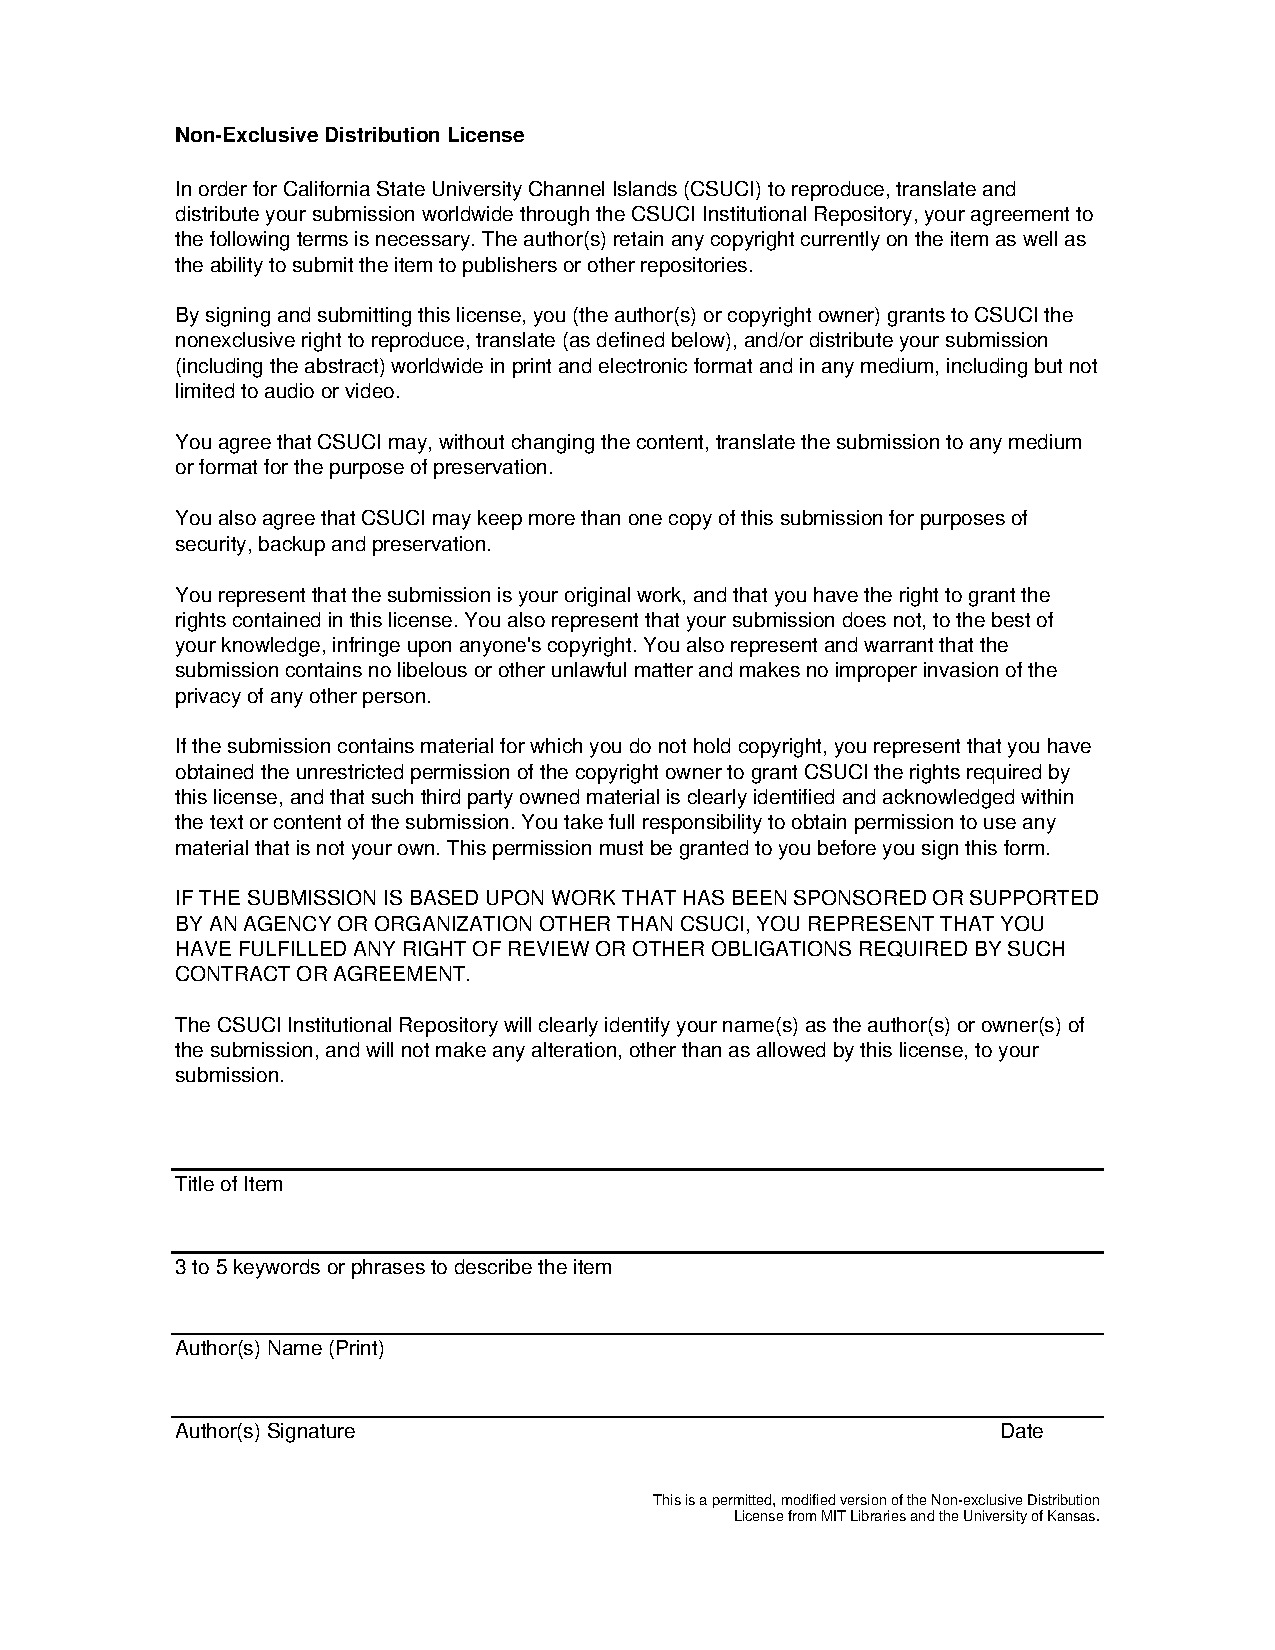
\includepdf{DistributionLicense.pdf}

\newpage

\title{Simplified and Inexpensive Mobile Digital Forensic Device} 
\author{Eric Elwood Gentry}

\date{\today}
\maketitle

\begin{abstract}
\end{abstract}

\newpage
\pagenumbering{roman}

\tableofcontents

\newpage

\listoffigures

\newpage
\pagenumbering{arabic}

\section{Abstract}
\label{sect-abstract}

\textbf{Keywords}: Digital Forensics, Triage, Mobile, Digital Evidence Backlog, Raspberry Pi

Goals: \\
\begin{itemize}
  \item preserve and protect evidenciary integrity
  \item reduce evidence gathering and triage analysis time
  \item prevent adding more to backlog than necessary by preventing over-confiscation
  \item reduce need for on-scene Digital Forensic Ssientists
  \item reduce backlog of digital evidence for tackling backlog
\end{itemize}

SEAKER tradeoffs: Precision (only relevant files) vs Recall (all relevant files)
- level of recall required at triage stage can be sacraficed\\

Introduce online storage system for digital forensic metadata format to enhance sharing capabilities across
jurisdiction boundaries and prevent sharing complexities

\section{Introduction}
\label{sect-intro}
\vspace{0.5 cm}

I know you are wondering what I am going to say here.  Your guess is as good as mine.  I really like
the introduction section, because I can say whatever I want! LOL\\

\section{Meetings with Frank}
\label{sect-frank}
\vspace{0.5 cm}
\subsection{May 18th, 2018}

My meeting with Frank Lyu, a civilian working for the Ventura County Sherriff's department, on loan to
the Southern California High Tech Task Force (SCHTTF) went well.  The SCHTTF is an 8 person team made up of
four civilians and four deputies, all reporting directly to the Ventura County District Attorney's office.
We met for lunch and I was able to ask him questions about the environment he works in as well as touch on
ranking the high value items that this SEAKER project could provide.\\

First, we talked about his work environment.  He has several responsibilities working for SCHTTF.  The first
and foremost is his caseload, which consists of examining digital evidence using forensic techniques in his
lab that result in a report to the District Attorney's office.  His other responsibilites include assisting
the District Attorney and staff with evaluating defense evidence reports, studying digital forensic 
technologies (for when he has to explain things to juries), helping other agencies identify and catalog
evidence that they are not familiar with, helping serve warrants on critical cases, and helping to retrieve
lost digital materials for other law enforcement agencies.

He explained that following the processes and procedures is by far the most important aspect of his job.  The
evidence handling, storage, and evaluation are critical to whether a case succeeds or is dismissed. Frank
began to describe the intake process, which involves the evidence, the agency report, and the search warrant
that will be used to search and evaluation the materials.  We did not go into further detail.

Items he looks for during an on-site warrant are: user accounts, previewing the materials (especially in
cases involving CP), and checking for the existence of Peer-to-Peer sharing utilities.  In addition, he 
strives to collect the following networking information: publically broadcast SSIDs, each SSID's level of
encryption, how many devices are connected to the router, and the external IP address for the router.

Value of SEAKER in the field: Filename search utilizing regular expression, the networking information 
specified in the last paragraph, producing a report, making an ios app instead of using a webpage, links
for the files found, and clickable thumbnails.

Value of SEAKER in the lab: Filename search utilizing regular expression and SEAKER hashes of images.  He
also mentioned a Microsoft tool called PhotoDNA that they currently use to find naked humans.

I asked about obtaining all of the statistics related to ingestion or evidence, caseload, pace at which
evidence can be evaluated, etc.  Frank's answer was that Adam could probably provide that information
without lab access, but that Michael should be asked to talk to Adam.

Finally, Frank mentioned that sometimes in financial cases, he is asked to search computers at business
offices, and the ability to search for specific filenames is very important there.

\newpage
\section{Background}
\label{sect-background}

\subsection{Review Material and Analysis}

\vspace{0.5 cm}
\textbf{Current challenges and future research areas for digital forensic investigation - Lillis et al., 2016 \cite{lillis2016current}}\\
\\

Some of the current challenges in digital forensic investigations are directly related to the amount of data being
created.  As Lillis et al\cite{lillis2016current} explores in their research, there are three main factors
involved in the digital forensic backlog: increasing number of devices seized per case, increased number of cases
involving digitial evidence, and the increasing volume of data per digital media.  This has lead to a growing
and already substantial backlog in digital forensic investigations.\\

One effect of this increased delay and backlog is that cases become inactive, waiting for new leads.  A more
aggressive approach to solving the backlog could help prevent dismissals, cold cases, and potentially more
societal harm from a corrupt investigation suspect.\\

Raghavan\cite{raghavan2013digital} has accumulated a list of 5 major challenges that the digital forensics 
community is facing and continue to add to the backlog problem.\\

The first is the complexity of binary data aquisition, i.e. low level data aquisition through digital media
duplication.  This challenge causes the need for sophisticated data reduction techniques.\\

Another complexity is the diversity of data and lack of standard examination techniques.  The plethora of
operating systems and file formats has been increasing and is posing a more and more significant challenge
over time.\\

The consistency and correlation problem is yet another challenge.  This is a problem resulting from the current
digital media investigation tools not providing the entire picture to investigators.  Only part of the whole
picture is provided when these tools find digital evidence.\\

Another issue that Raghavan\cite{raghavan2013digital} proposed is the volume of data to sort through.  The sheer
amount of data that exists per user is increasing at an alarming rate [cite?], and has lead to a very large
backlog of digital evidence to investigate.  These delays have even caused some cases to be dismissed.  This
challenge is exacerbated by the lack of adequate automation for digesting the data.\\

The fifth, but certainly not the last, challenge proposed by Raghavan\cite{raghavan2013digital} is the timeline
synchronization issue with digital evidence.  Since the evidence could be collected in different time zones, 
with different timestamp formats, clock skew, etc, lining up the events in order can be challenging or
infeasible.\\

With the proliferation of Internet Of Things (IOT) devices and cloud storage, the field of digital forensics
continues to expand.  These areas pose a great challenge, but also new opportunities.  Lillis et
al\cite{lillis2016current} researched cloud storage and found some areas of opportunity, for instance parallel
processing, distibuted computing, GPU/FPGA utilization, and others.  These areas for increasing the efficiency
of ditigal forensics can be explored further due to the substantially reduced I/O limitations in cloud storage.\\

The Internet of Things (IOT) also poses new challenges.  IOT devices are estimated to number near 40 billion by
2020, contributing to the overwhelming amount of digital data.  Since these devices tend to have more 
non-persistent memory and less storage, this causes added complexity for gathering and analysis.  In addition,
a portion of IOT devices are battery operated and computationally challenged, leading to loss of data over
time.\\
\vspace{0.5 cm}

\textbf{Tiered forensic methodology model for Digital Field Triage by non-digital evidence specialists - Hitchcock et al., 2016\cite{hitchcock2016tiered}}\\
\\

Hitchcock et al\cite{hitchcock2016tiered} has proposed and evaluated a "tiered forensic methodology" model that defines
a process of digital forensic triage utilizing non-digital evidence specialists.  In their research, they identified
a large and growing backlog of digital evidence.  This backlog has led to problems in the law enforcement community
with regards to collecting, analyzing, reporting, and prosecuting.\\

The summary of the research done by Hitchcock et al\cite{hitchcock2016tiered} are as follows.  They sought to expedite
the process of sending digital evidence for analysis and results.  One of their goals is to enable more field triage
of digital evidence to reduce the amount collected, and act specifically on pertinent information only.  They 
recommended that some front-line crime scene investigators (non-forensic analysts) be trained in the implementation
of digital evidence triage and evaluation.  These trained individuals would be Digital Field Triage (DTF) experts and
have the ability perform field-level digital evidence triage.  This triage would specifically weed out the benign
from the consequential digital evidence with high certainty, while also protecting the digital evidence from spoilage
and preserving evidentiary integrity.\\

The next tier is where the already-triaged digital evidence is sent for full evaluation.  This is a certified facility
that can perform full digital forensic analysis, called a Technological Crime Unit (TCU).  The TCU is currently
heavily inundated with cases needing analysis and reporting of digital evidence.\\

The backlog and delays in case reporting are contributors to a common problem of time sensitivity.  Some countries 
have given their citizens a right to a "speedy" trial.  As well, some countries have statutes of limitation (limits
on how long after the crime was committed to resolve the case) for most crimes.  Some administrative situations are
also contributors, for instance case prioritization based on chronological filing, crime severity, or victim needs.\\

This tiered approach is based on a Computer Forensic Field Traige Process Model proposed by Rogers et al
\cite{rogers2006computer} and the internation standard ISO 27037 (Information Technology - Security Techniques - 
Guidelines for identification, collection, aquisition, and presentation of digital evidence). The process model 
breaks down the six phases of digital evidence categorization, which Hitchcock et al\cite{hitchcock2016tiered} loosely
based their four phase approach on.  The four phases are: planning, assessment, reporting, and threshold.  The ISO
27037 standard specifically attempts to address the need to minimize the risk of potential digital evidence being
spoiled by mis-handling, while also attempting to maximize the evidentiary value of digital evidence collection.\\

This approach is not without risks.  One concern is the accidental exclusion of an item of digital evidence that is
important to the investigation.  Another is the level of computer skills and training of the DTF expert.  The paper
does attempt to mitigate the latter with training and management process, while providing evidence that the former
is a common misconception in most cases.\\

The research of Hitchcock et al\cite{hitchcock2016tiered} should be referenced for a good process starting point for
digital forensic labs.
\vspace{0.5 cm}

\textbf{A practical and robust approach to coping with large volumes of data submitted for digital forensic examination \cite{shaw2013practical}}\\
\\

One digital evidence triage method proposed by Shaw et al\cite{shaw2013practical} seeks to standardize on an 
approach they call "enhanced previewing".  Enhanced previewing seeks to solve some of the problems associated with
typical triage approaches.  As is the case in other research, Shaw et al\cite{shaw2013practical} extolls the 
need to reduce digital forensic evidence analysis backlogs, especially with the evolution of big data and the
proliferation of digital devices.\\

Shaw et al\cite{shaw2013practical} points out that neither digital forensic triage examination nor digital forensic
full examination are well defined.  Triage may mean something completely different to two digital forensic
examiners.  As well, full digital forensic examination has no robust standard to follow.\\

The proposal for a practical and robust method by Shaw et al\cite{shaw2013practical} aims to stem the concerns
of a typical triage process.  Risks still exist, for instance overlooking digital evidence, but it is argued that
those risks are outweighed by the risks of a lengthy process due to large backlogs and the associated delays in
evaluating that evidence.  Another concern esists that inadequately trained people will be charged with performing
on-site digital evidence triage and mishandling or incorrectly evaluating results will cause evidence spoilage.
Other concerns are the potential high cost of software and training.\\

In order to provide a simple, yet robust mechanism, Shaw et al\cite{shaw2013practical} starts with an open source,
CD-bootable image of GNU/Linux and enhances its features to include boot-time application launching, and a simple
to use interface with minimal ability to deviate from task.  This bootable CD is intended to be placed into 
evidenciary computer systems and booted using a series of BIOS modifications or boot-time interruptions.  This 
mechanism to boot the system off of a bootable CD is difficult, and where the most problems with untrained users
of the enhanced previewing will happen.\\

The enhanced previewing concept has valuable merit, in that the collection mechanisms are thorough.  Using the
GNU/Linux based system and having written code for it, Shaw et al\cite{shaw2013practical} utilized some well
thought-out approaches.  First, all hard drives from the evidentiary system are mounted into the GNU/Linux
filesystem as read-only, thereby obviating the need for write-blockers.  As well, the entire hard drive is
evaluated, including the file system, all partitions, unallocated space, deleted files, and compressed files.  In
addition, other mechanisms are employed that continue to enhance the previewing are employed.  One example is to
note encrypted compressed files for review later.\\

They also strongly compliance with digital forensics best practices, like the ones provided in the ACPO.  This
standards guide is from the UK and is titled Best Practices Guide for Digital Evidence (2012).  There are four
main practices outlined, but the main one that Shaw et al\cite{shaw2013practical} chose to point out was the
second one regarding the integrity protection of the original digital media.
\vspace{0.5 cm}

\textbf{Computer Forensics Field Triage Process Model - Rogers et al., 2006\cite{rogers2006computer}}\\
\\

Rogers et al\cite{rogers2006computer} proposed a reliable, repeatable process model in 2006 for digital evidence
triage in the field.  It was created in partnership with Purdue University Cyber Forensics and Computer and Information
Technology Departments, along with the National White Collar Crime Center <NEED CITE>.  The process is derived from
several other models including Integrated Digital Investation Process model (IDIP), Digital Crime Scene Analysis (DCSA),
and a military Operations Order (OpOrd).  In coordination with the Southern Indiana Assistant U.S. Attorney's office,
USADA Steve Debrota, Rogers et al\cite{rogers2006computer} implemented and reported on the success of their proposed
model: Computer Forensics Field Triage Process Model (CFFTPM).\\

The CFFTPM was created to enhance the investigators ability to obtain useful information at execution time of a 
warrant at the suspect's dwelling or work.  The process is designed to be used in the first few hours of the 
investigation, especially udring the first suspect interview and search execution phase of the investigation.  It is
known that suspects are more likely to divulge more information and be more cooperative in that environment (Yeschke
2003\cite{yeschke2003art}).  As well, location of and presentation with suspect "triggers" from the potential evidence
increase the suspect's willingness to talk and cooperate while on site. <NEED CITE>.\\

The foci of the CFFTPM are immediately finding usable evidence, identifying victims at acute risk, guiding the
on-going investigation, identify potential charges, and accurately assess the offender's danger to society.  In
addition, the process is intended to protect the integrity of the evidence or potential evidence in an investigation.
This process in no way supersedes the ability or need to perform a full forensic examination at a full-featured
digital forensic lab.\\

The CFFTPM is broken up into phases that have sub-phases (see Figure 1).  The main phases consist of Planning, Triage, Usage/User
Profiles, Chronology/Timeline, Internet Activity, and Case-Specific Evidence.  The primary machine type that this model
covers is the standard Windows machine.  Usage/User Profiles are broken down into three sub-phases: Home Directory,
File Properties, and Registry.  These are important and help distinguish user specific activity and permissions.  The
Internet Activity phase is also broken down into three sub-phases: Browser Artifacts, Email Artifacts, and Investation
Messenger Artifacts.  These also help establish user activity.  Some importance is explicitly stated to skip based on
type of investigation and prioritizing the investigation.  This is where the SEAKER portable triage device can help by
evaluating every aspect and prevent the on-site investigators from skipping or de-prioritizing critical potential
evidence.\\

\begin{figure}[h]
  \centering
    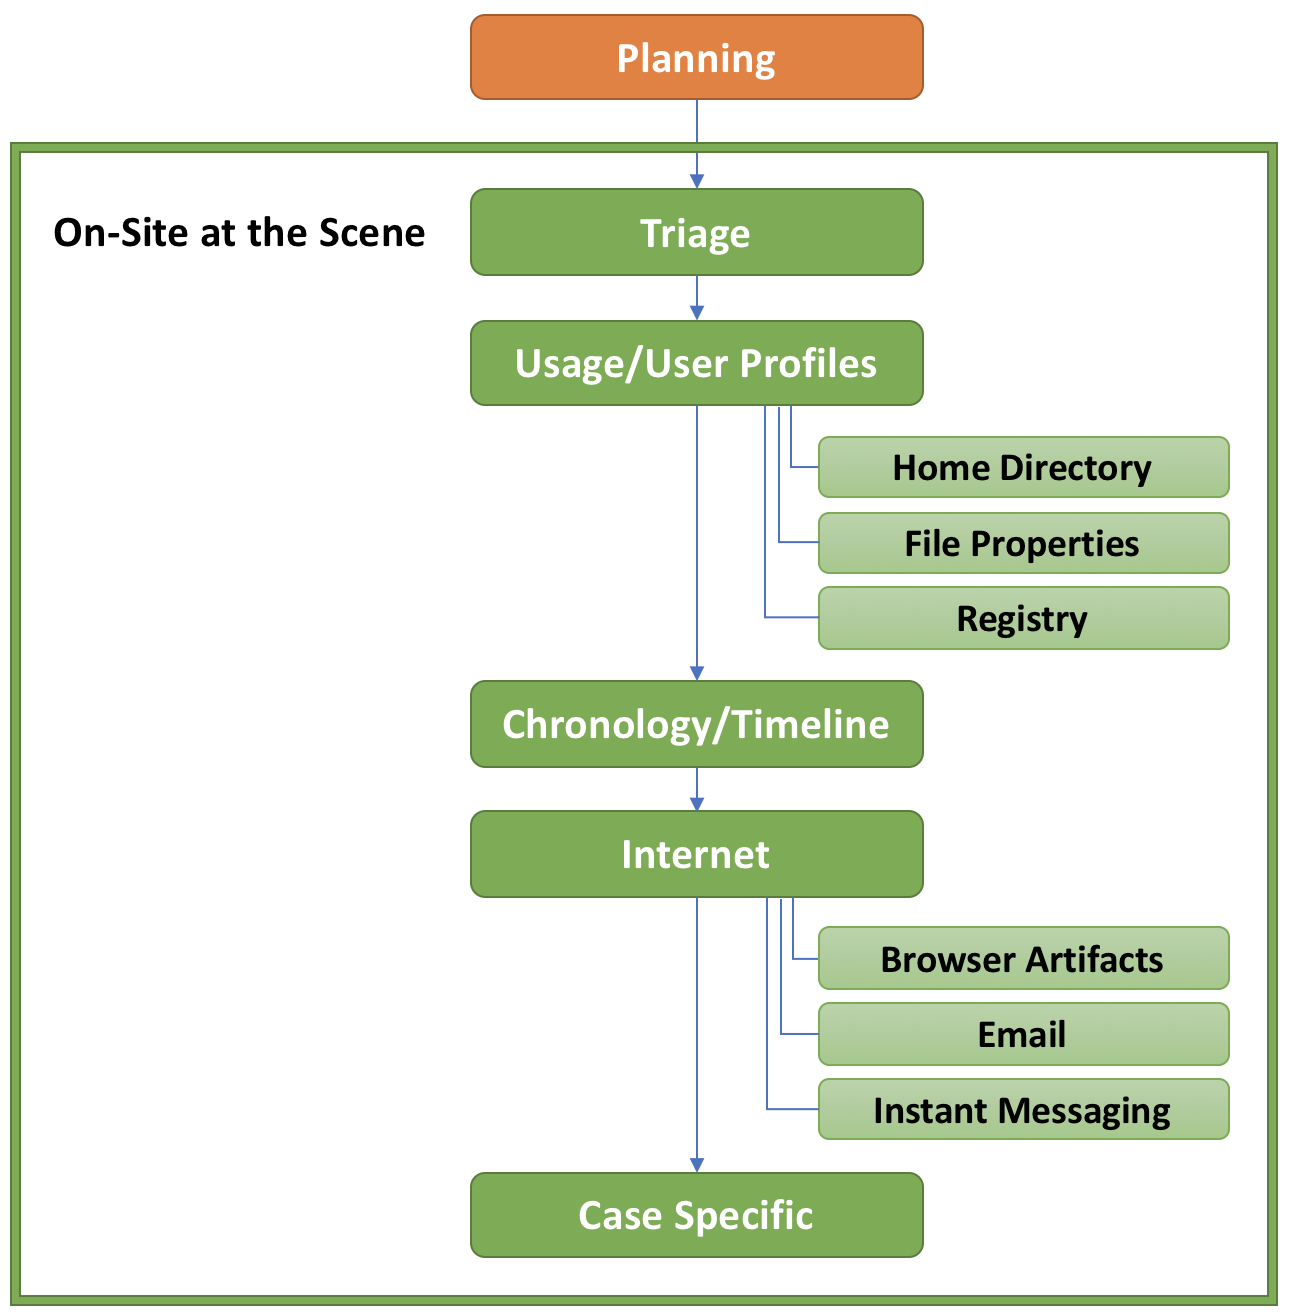
\includegraphics[width=0.8\textwidth]{CFFTPM.png}
  \caption{Computer Forensic Field Triage Process Model (CFFTPM)}
\end{figure}

The authors of the CFFTPM (Rogers et al\cite{rogers2006computer}) also note the important legal and technical
considerations prior to implementing CFFTPM on a particular investigation.  The legal considerations include issues
related to search warrant scope and limitations, U.S. Constitutional 4th Amendment rights, etc.  The technical 
considerations include type of case, criticality of timeliness, skillset of the on-site digital forensic examiner, 
skillset of the suspect, having proper lab equipment on-site, scene control, etc.  This is also an area where the
SEAKER portable triage device can help eliminate some of the potential problems, for instance technical prowess of the
on-site investigators and proper lab equipment on-site.\\

Some particular aspects of the phases are critical to investigators in revealing evidence or potential evidence for
the SEAKER portable traige device.  Usage/User Profile information is extremely important.  This includes the need to
be able to view and search files, folders, registry keys, and file properties associated with a particular user.  The
Internet Activity artifacts also become very useful, especially in the case of child pornography.  The browser, email,
and Instant Messaging artifacts can lead directly to potential charges.  Finally, a Chronology/Timeline understanding
and ability to sort based on it can significantly narrow down the possibilities of which user information and which
Internet Activity is the most important and critical to the investigation.\\

Implementing this in the SEAKER portable triage device is crucial for simplicity and ease of use.  As well, it goes a
long way towards having an implementation of SEAKER being understood and adopted.  Reporting is also a critical need
and is implemented in a way that will enable digital forensic investigators to provide early information to
investigators and prosecutors.  This helps alleviate the need to wait until the backlog of digital evidence is cleared
to get any information from case-specific digital evidence.
\vspace{0.5 cm}

\textbf{The design science research process: a model for producing and presenting information systems research - Peffers et al., 2006\cite{peffers2006design}}\\
\\
\vspace{0.5 cm}

\textbf{Testing the harmonised digital forensic investigation process model-using an Android mobile phone \cite{omeleze2013testing}}\\
\\
\vspace{0.5 cm}

\textbf{Forensic analysis of iPhone backups \cite{satishforensic}}\\
\\
\vspace{0.5 cm}

\textbf{Forensic analysis of social networking applications on mobile devices \cite{al2012forensic}}\\
\\
\vspace{0.5 cm}

\textbf{Jailbroken iPhone Forensics for the Investigations and Controversy to Digital Evidence \cite{chang2015jailbroken}}\\
\\
\vspace{0.5 cm}

\textbf{Methods and tools of digital triage in forensic context: survey and future directions \cite{jusas2017methods}}\\
\\
\vspace{0.5 cm}

\textbf{A survey of digital forensic investigator decision processes and measurement of decisions based on enhanced preview \cite{james2013survey}}\\
\\
\vspace{0.5 cm}

\textbf{Forensic examination of digital evidence: a guide for law enforcement \cite{hart2004forensic}}\\
\\
\vspace{0.5 cm}

\section{SEAKER Creation}
\label{sect-Creation}
See Figure 2.
  \begin{figure}[h]
    \centering
      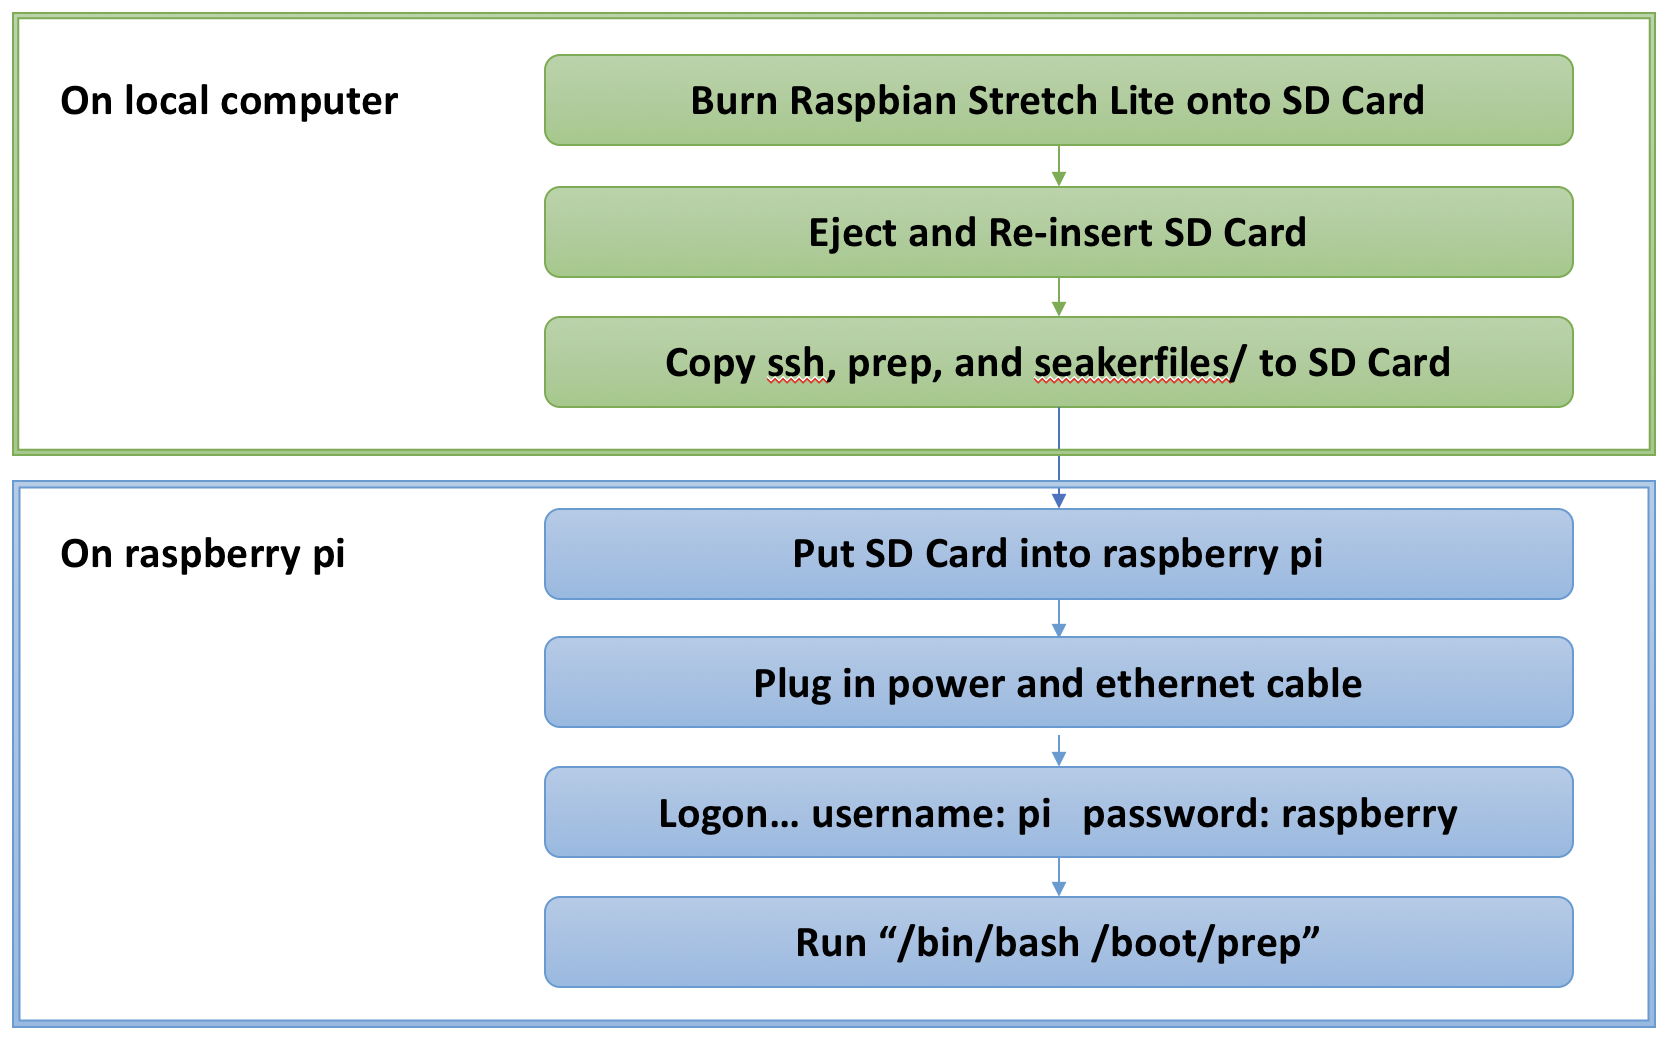
\includegraphics[width=0.8\textwidth]{SeakerCreation.png}
    \caption{SEAKER Creation Process}
  \end{figure}

\section{Analysis}
\label{sect-analysis}

\subsection{Process for gathering digital evidence}

First of all, never boot a computer.  That will alter the original state of the hard drive due to the operating
system being loaded.  This may alter the data available for collection and render the digital media "spoiled" and
therefore unusable ad evidence in a case.\\

The main point here is to preserve evidentiary integrity and protect against spoilage.\\

Specific training is required to be able to handle digital evidence properly.  What do digital evidence collectors
already have to go through in terms of training?\\

\subsection{SEAKER Usage Methodologies}
\subsubsection{Connected Method}

In this approach, SEAKER is hard-wired using an ethernet cable to the internet or the lab intranet.  The connection
is utilized to connect directly to the Image Hash Storage Server (IHSS) and the Digital Evidence Storage Server (DESS).
The digital evidence is still collected locally, but also being transmitted to the DESS and comparing image hashes
to the IHSS.\\

\subsubsection{Disconnected Method}

In this approach, SEAKER is not connected to an ethernet cable and is solely being used as a wifi router for
collecting digital evidence locally.  A unique digital collection ID will be created when connected to the DESS
at a later time.

\subsection{Automated processes during SEAKER evaluation}

\subsubsection{Local processing}

This section describes the local processing that takes place in both Connected and Disconnected Methods.
\begin{itemize}
  \item picture of digital media
  \item picture of hosting hardward platform (laptop, computer, server, phone, etc)
  \item file list
  \item full log of capturing/viewing/analysis
  \item image thumbnails
  \item video thumbnails
  \item browser history
  \item emails
  \item user profiles
  \item deleted files
  \item image thumbnail subsets (images with faces, bodies, documents, etc)
  \item searches performed
  \item anything "marked" as an "artifact"
\end{itemize}

\subsubsection{Remote processing}

This section describes the remote processing that takes place only when Connected Method is in use.
\begin{itemize}
  \item matching hashes of images
  \item matching hashes of videos
  \item online storage of digital evidence collection for this case at this site and time
\end{itemize}

\newpage
\section{Conclusion and future work}
\label{sect-conclusion}

My conclusion is going to be very fascinating and wonderful.  I can feel it.

\subsection{Future work}
\begin{itemize}
  \item Online hard drive investigation (i.e. Cloud Forensics)
  \item Network Traffic Investigation
  \item Video segmentation and video image hashing
  \item crime-specific searchs:
  \begin{itemize}
    \item financial crimes
    \item credit card fraud
    \item hacking
    \item bullying
    \item bloackmail
    \item espianage
    \item fraud
    \item customizable (corporate / military)
  \end{itemize}
  \item OS lockdown (raspbian)
  \item phone specific OS tools
  \item phone specific apps
  \item encrypted devices (password entry location, assessment without password)
  \item running machine RAM assessment
  \item utilize forensics as a service
\end{itemize}

\newpage
\section{Code improvements}
\begin{itemize}
  \item Query Expansion - automatically searching for same query maybe other contexts
  \item Synonym Matching - automatically searching for similar words to query word
  \item collect everything in UTC time
  \item universal way of collecting hard drive hash for verification of evidence integrity
  \item Data Visualizations:
  \begin{itemize}
    \item present all data visualizations for particular drive or all hard drives
    \item graph - size vs amount of files (one hard drive, and all hard drives)
    \item graph - common details (like file type, etc) maybe clickable!
    \item graph/chart - files by date
    \item graph/chart - files by file type
    \item chart - website visits
    \item digital image hashes list (stored and compared)
  \end{itemize}
  \item for analysis: skip OS files, applications files, etc
  \item lock down OS
  \item Investigation Gathering rollup: (stored online)
  \begin{itemize}
    \item Database Schema
    \item metadata
    \item Unique "gathering ID"
    \item case number
    \item observation report
    \item crime severity
    \item potential offenses
    \item time gathered
    \item gatherer
    \item suspect list
    \item location gathered
    \item suggestions for other research
    \item which computer system it came from
    \item SET of evidence
    \item Digital Evidence item
    \item images of item
    \item unique item ID
    \item file contents
    \item ranking within set of evidence
    \item image thumbnails
    \item collection statistics
    \item etc
  \end{itemize}
  \item swap file review
  \item find encryption Keys 
  \item bulk extractor ? 
  \item thumb strips of movies
  \item predetermine search criteria (passwords, pw, etc)
  \item encrypted password entry?
  \item get file owner, MAC times
  \item sort based on user
  \item sort based on access time
  \item read registry file (make available for search)
  \item time search i.e. time=lastweek, time=5/5/18-5/15/18
  \item internet usage timeline
  \item autosearch/autofilter
  \item email search
  \item for drug search... Spreadsheets, documents, databases, internet purchase strives
  \item for financial search... Spreadsheets, databases, MSMoney, Quicken

\end{itemize}

\newpage
\section{Keywords and glossary}
\begin{itemize}
  \item Contraband files
  \item stages: preprocessing, storage, analysis, reporting
  \item stages: gather (document, catalog), triage (analyze, live review, automated review, artifact storage,
  meet threshold?), results (present, graphs, search)
  \item Chain of Custody for digital evidence
  \item Forensic integrity of digital evidence
  \item artifacts = pieces of digital evidence that are of importance to the case
  \item enhanced previewing - better than triage (full drive)
  \item Indecent Image of Children
  \item Image Hash Databases - dbs of digital forensic labs with image hashes
  \item obviate the need for write blockers
  \item early look intelligence gathering
  \item Immediate feedback loop for onsite investigators
  \item "Suspect's dwelling"
  \item securing a conviction of the offender
  \item protecting future victims
  \item browser artifacts
  \item onsite == in situ
  \item adhere to proven forensic principles
\end{itemize}

\newpage
\section{Graphs, Images, Figures, and tables}
\begin{itemize}
  \item figure - field triage flowchart
  \item figure - each stage field triage flowchart
  \item figure - Image analysis and hash creation flowchart
  \item graph - aquisition time vs full
  \item graph - investigation time vs full
  \item graph - analysis time vs full
  \item graph - total time from initial plug-in to decision to be evidence (threshold)
  \item graph - current backlock in ventura county
  \item figure - DFT vs TCU (Hitchcock\cite{hitchcock2016tiered})
  \item graph - collection time vs number and size of files
  \item figure - see figures in Computer Forensic Field Triage Process model (Rogers)

\end{itemize}

\newpage
\bibliographystyle{plain}
\bibliography{references}

\end{document}

